% Corrected FETP stock-and-flow and causal-loop diagrams.
% Two standalone PDF pages: panel (a), then panel (b).
% Compile in a complete TeX installation (or Overleaf):
%   pdflatex FETP_corrected_diagrams.tex
% Manuscript inclusion:
%   \includegraphics[page=1,width=\textwidth]{FETP_corrected_diagrams.pdf}
%   \includegraphics[page=2,width=\textwidth]{FETP_corrected_diagrams.pdf}
% Required packages: standalone, fontenc, lmodern, amsmath, tikz.
% The diagram describes the default benchmark: advanced + intermediate.
% It is a schematic of the supplied fetp_model-3.py, not a claim that
% the feedback parameters have been empirically estimated.
\documentclass[border=5pt,multi=tikzpicture]{standalone}
\usepackage[T1]{fontenc}
\usepackage{lmodern}
\usepackage{amsmath}
\usepackage{tikz}
\usetikzlibrary{arrows.meta,positioning,calc,shapes.symbols,backgrounds}

\definecolor{ink}{HTML}{243247}
\definecolor{stockfill}{HTML}{EEF2F7}
\definecolor{flowcol}{HTML}{39506F}
\definecolor{rcol}{HTML}{A73B32}
\definecolor{bcol}{HTML}{216B86}
\definecolor{postcol}{HTML}{34704D}
\definecolor{muted}{HTML}{596574}
\definecolor{edge}{HTML}{BBC3CC}

\tikzset{
  stock/.style={draw=ink,fill=stockfill,line width=.9pt,
    minimum width=29mm,minimum height=12mm,align=center,
    inner sep=4pt,font=\sffamily\small,text=ink},
  aux/.style={draw=edge,fill=white,rounded corners=2pt,
    align=center,inner sep=4pt,font=\sffamily\small,text=ink},
  cloudnode/.style={cloud,cloud puffs=10,cloud puff arc=120,
    aspect=2,draw=edge,fill=white,minimum width=17mm,
    minimum height=10mm,align=center,font=\sffamily\scriptsize},
  flow/.style={draw=flowcol,line width=1.6pt,-{Latex[length=2.8mm]}},
  info/.style={draw=muted,line width=.65pt,-{Latex[length=2mm]}},
  causal/.style={line width=.85pt,-{Latex[length=2.3mm]}},
  lab/.style={font=\sffamily\scriptsize,align=center,
    fill=white,inner sep=2pt,text=ink},
  note/.style={font=\sffamily\small,align=left,text=muted},
  sign/.style={font=\sffamily\small\bfseries,fill=white,inner sep=1.5pt},
  title/.style={font=\sffamily\bfseries,anchor=west,text=ink},
  loopnode/.style={aux,minimum width=29mm,minimum height=13mm},
  badge/.style={circle,draw,line width=1pt,fill=white,
    minimum size=9mm,font=\sffamily\small\bfseries},
  pics/valve/.style={code={
    \filldraw[draw=flowcol,fill=white,line width=.7pt]
      (-1.5mm,-1.1mm)--(1.5mm,1.1mm)--(1.5mm,-1.1mm)--(-1.5mm,1.1mm)--cycle;
  }}
}

\begin{document}

% =====================================================================
% PANEL (a): workforce accounting. Course records and people are separate.
% =====================================================================
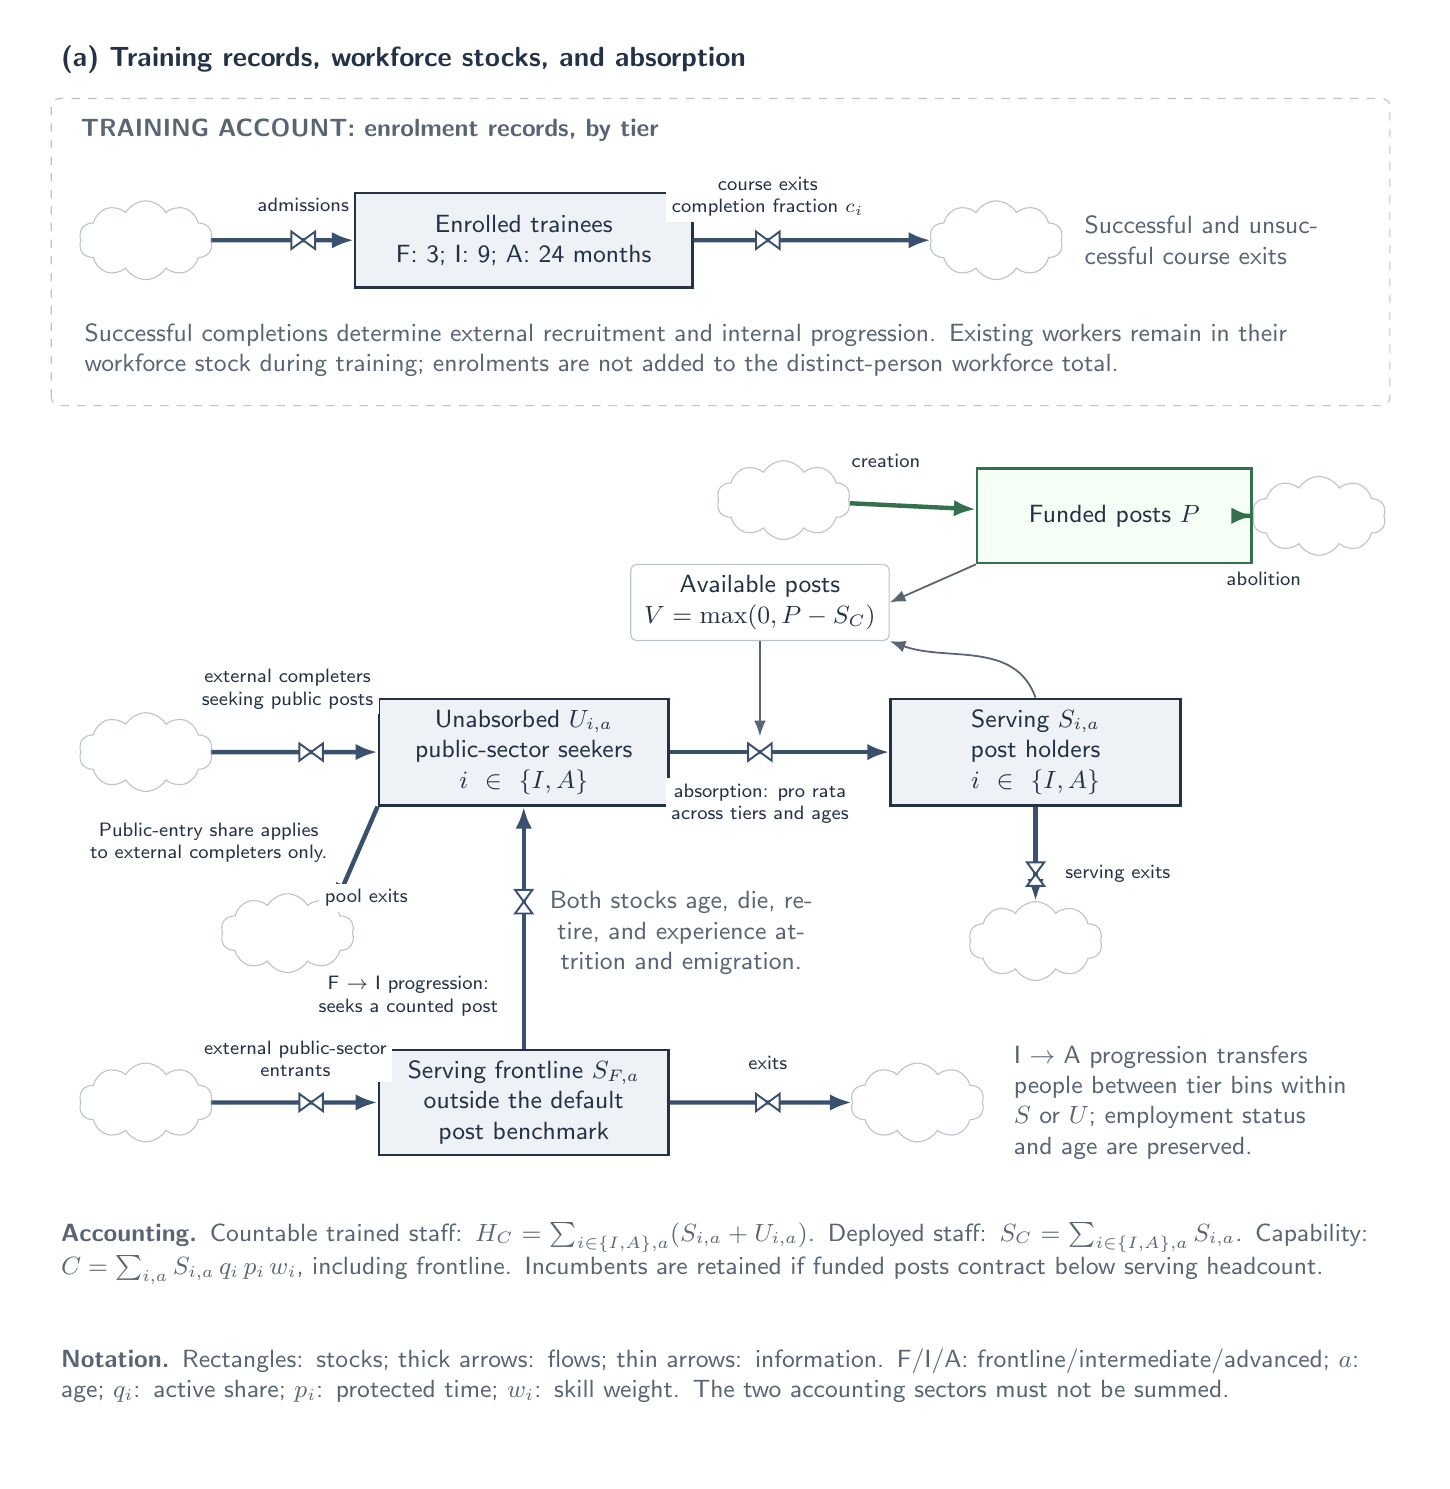
\begin{tikzpicture}[x=1cm,y=1cm,font=\sffamily]
\path[use as bounding box] (-.3,-1.2) rectangle (17.4,17.0);
\node[title] at (0,16.6) {(a) Training records, workforce stocks, and absorption};

% Training queues count enrolments; internal trainees also remain in their
% workforce stock until completion. They are not additional distinct people.
\draw[draw=edge,dashed,rounded corners=3pt] (0,12.2) rectangle (17,16.1);
\node[note,anchor=west,font=\sffamily\small\bfseries] at (.25,15.7)
  {TRAINING ACCOUNT: enrolment records, by tier};
\node[cloudnode] (applications) at (1.2,14.3) {};
\node[stock,text width=40mm] (training) at (6.0,14.3)
  {Enrolled trainees\\F: 3; I: 9; A: 24 months};
\node[cloudnode] (courseend) at (12.0,14.3) {};
\draw[flow] (applications)--(training);
\pic at (3.2,14.3) {valve};
\node[lab] at (3.2,14.75) {admissions};
\draw[flow] (training)--(courseend);
\pic at (9.1,14.3) {valve};
\node[lab] at (9.1,14.85) {course exits\\completion fraction $c_i$};
\node[note,anchor=west,text width=35mm] at (13.0,14.3)
  {Successful and unsuccessful course exits};
\node[note,anchor=west,text width=160mm] at (.3,12.9)
  {Successful completions determine external recruitment and internal progression.
   Existing workers remain in their workforce stock during training; enrolments
   are not added to the distinct-person workforce total.};

% Funded establishment is a separate stock, not a stock of people.
\node[stock,draw=postcol,fill=green!4,text width=32mm] (posts) at (13.5,10.8)
  {Funded posts $P$};
\node[cloudnode] (postsource) at (9.3,11.0) {};
\node[cloudnode] (postsink) at (16.1,10.8) {};
\draw[flow,draw=postcol] (postsource)--(posts);
\node[lab] at (10.6,11.5) {creation};
\draw[flow,draw=postcol] (posts)--(postsink);
\node[lab] at (15.4,10.0) {abolition};
\node[aux,text width=30mm] (vacancy) at (9.0,9.7)
  {Available posts\\$V=\max(0,P-S_C)$};
\draw[info] (posts.south west)--(vacancy.east);

% Counted workforce: explicit age-structured unabsorbed and serving stocks.
\node[cloudnode] (ext) at (1.2,7.8) {};
\node[stock,text width=34mm] (pool) at (6.0,7.8)
  {Unabsorbed $U_{i,a}$\\public-sector seekers\\$i\in\{I,A\}$};
\node[stock,text width=34mm] (serving) at (12.5,7.8)
  {Serving $S_{i,a}$\\post holders\\$i\in\{I,A\}$};
\draw[flow] (ext)--(pool);
\pic at (3.3,7.8) {valve};
\node[lab] at (3.0,8.6) {external completers\\seeking public posts};
\draw[flow] (pool)--(serving);
\pic at (9.0,7.8) {valve};
\node[lab] at (9.0,7.15) {absorption: pro rata\\across tiers and ages};
\draw[info] (vacancy.south)--(9.0,8.0);
\draw[info] (serving.north) to[out=110,in=-20] (vacancy.south east);
\node[lab] at (2.0,6.65) {Public-entry share applies\\to external completers only.};

\node[cloudnode] (upoolloss) at (3.0,5.5) {};
\node[cloudnode] (sloss) at (12.5,5.4) {};
\draw[flow] (pool.south west)--(upoolloss.north east);
\node[lab] at (4.0,5.95) {pool exits};
\draw[flow] (serving)--(sloss);
\pic[rotate=90] at (12.5,6.25) {valve};
\node[lab,anchor=west] at (12.8,6.25) {serving exits};
\node[note,text width=48mm,align=center] at (8.0,5.5)
  {Both stocks age, die, retire, and experience attrition and emigration.};

% Frontline is not post constrained under the default benchmark.
\node[cloudnode] (fsource) at (1.2,3.35) {};
\node[stock,text width=34mm] (front) at (6.0,3.35)
  {Serving frontline $S_{F,a}$\\outside the default\\post benchmark};
\node[cloudnode] (floss) at (11.0,3.35) {};
\draw[flow] (fsource)--(front);
\pic at (3.3,3.35) {valve};
\node[lab] at (3.1,3.9) {external public-sector\\entrants};
\draw[flow] (front)--(floss);
\pic at (9.1,3.35) {valve};
\node[lab] at (9.1,3.85) {exits};
\draw[flow] (front.north)--(pool.south);
\pic[rotate=90] at (6.0,5.9) {valve};
\node[lab,anchor=east] at (5.75,4.7) {F $\to$ I progression:\\seeks a counted post};
\node[note,anchor=west,text width=43mm] at (12.1,3.35)
  {I $\to$ A progression transfers people between tier bins within $S$ or $U$;
   employment status and age are preserved.};

\node[note,anchor=north west,text width=167mm] at (0,1.95)
  {\textbf{Accounting.} Countable trained staff:
   $H_C=\sum_{i\in\{I,A\},a}(S_{i,a}+U_{i,a})$.
   Deployed staff: $S_C=\sum_{i\in\{I,A\},a}S_{i,a}$.
   Capability: $C=\sum_{i,a}S_{i,a}\,q_i\,p_i\,w_i$, including frontline.
   Incumbents are retained if funded posts contract below serving headcount.};
\node[note,anchor=north west,text width=167mm] at (0,.35)
  {\textbf{Notation.} Rectangles: stocks; thick arrows: flows; thin arrows:
   information. F/I/A: frontline/intermediate/advanced; $a$: age;
   $q_i$: active share; $p_i$: protected time; $w_i$: skill weight.
   The two accounting sectors must not be summed.};
\end{tikzpicture}

% =====================================================================
% PANEL (b): signed causal loops. Signs are local, all else held constant.
% =====================================================================
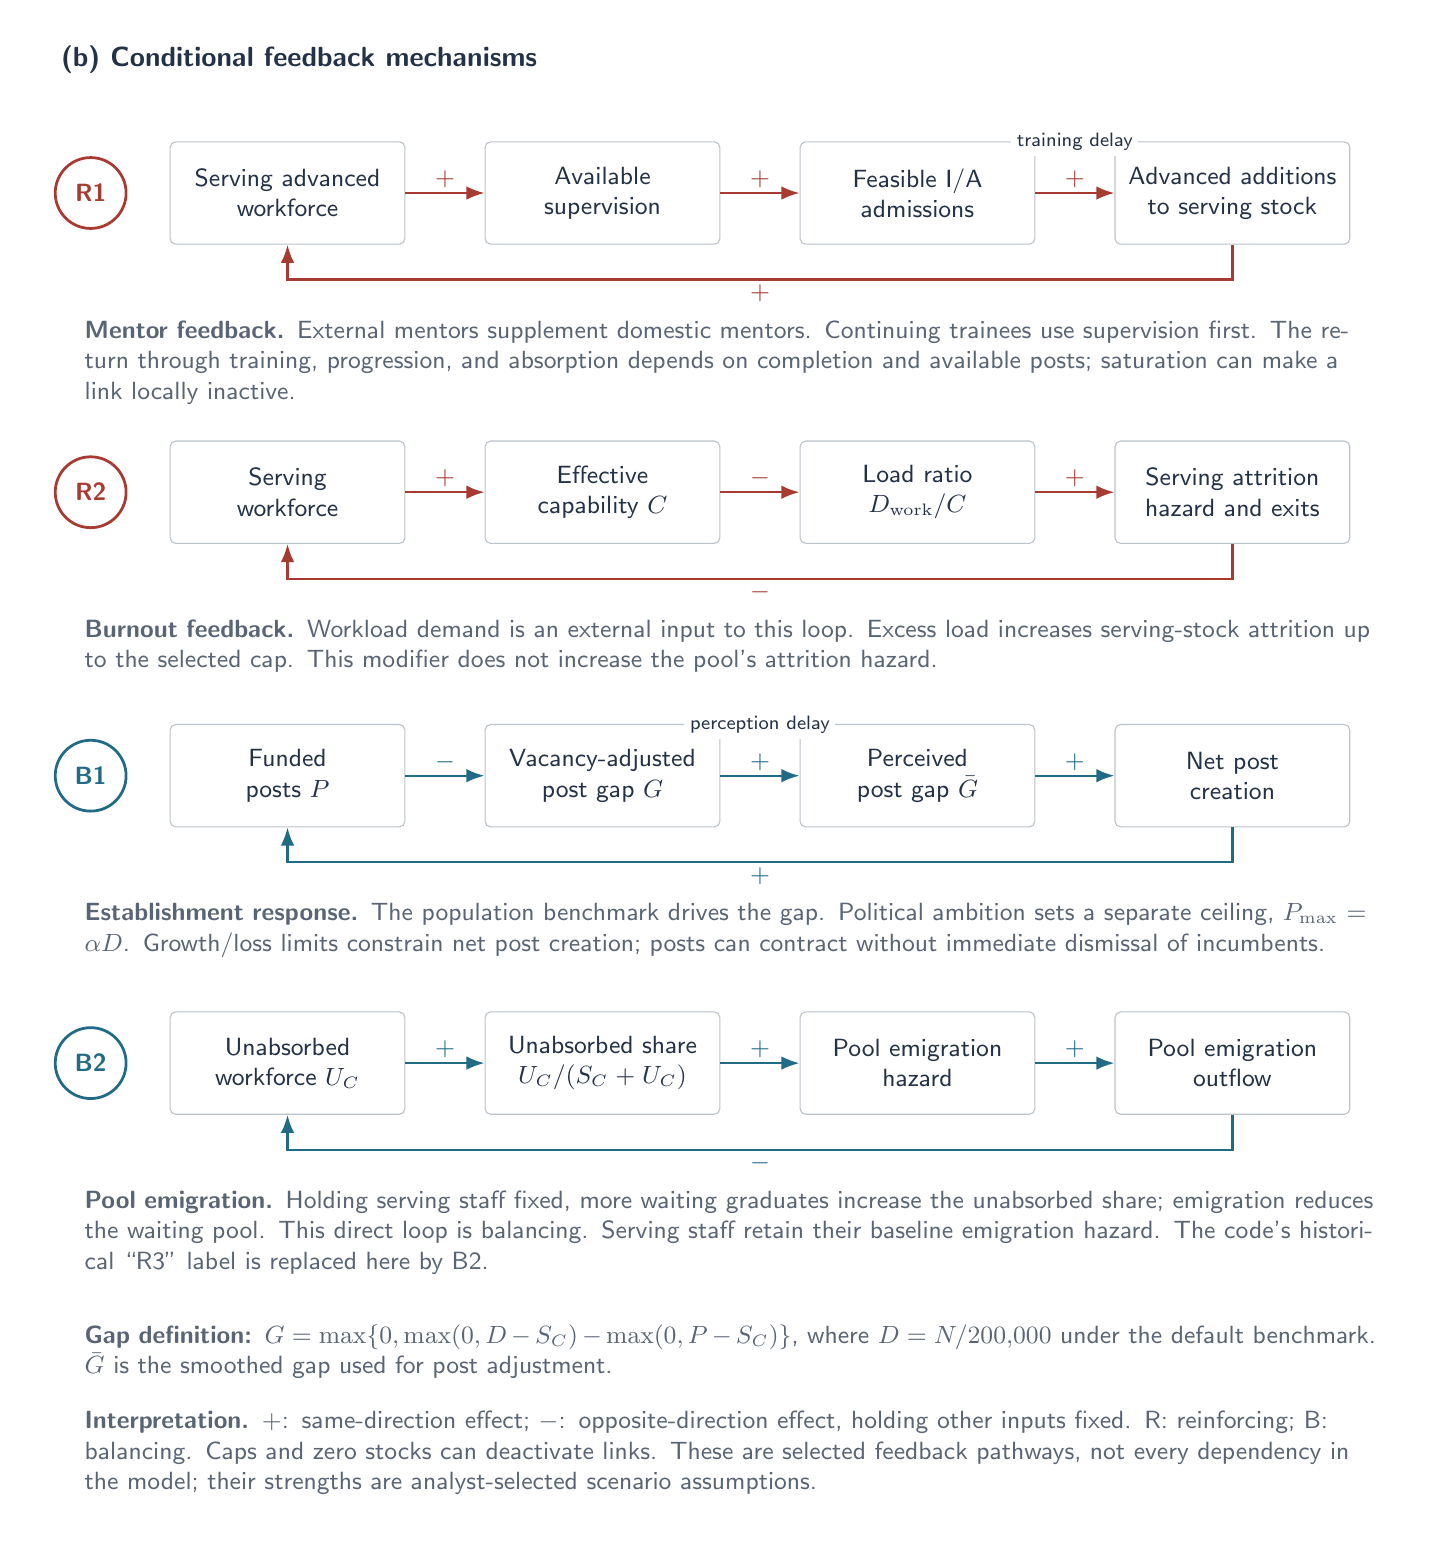
\begin{tikzpicture}[x=1cm,y=1cm,font=\sffamily]
\path[use as bounding box] (-.3,-2.2) rectangle (17.4,16.8);
\node[title] at (0,16.4) {(b) Conditional feedback mechanisms};

% R1: two positive accumulation links close a reinforcing training loop.
\node[badge,text=rcol,draw=rcol] at (.5,14.7) {R1};
\node[loopnode,text width=27mm] (a1) at (3.0,14.7) {Serving advanced\\workforce};
\node[loopnode,text width=27mm] (a2) at (7.0,14.7) {Available\\supervision};
\node[loopnode,text width=27mm] (a3) at (11.0,14.7) {Feasible I/A\\admissions};
\node[loopnode,text width=27mm] (a4) at (15.0,14.7) {Advanced additions\\to serving stock};
\draw[causal,rcol] (a1)--node[sign,above]{$+$}(a2);
\draw[causal,rcol] (a2)--node[sign,above]{$+$}(a3);
\draw[causal,rcol] (a3)--node[sign,above]{$+$}(a4);
\node[lab] at (13,15.35) {training delay};
\draw[causal,rcol] (a4.south)--(15,13.6)--node[sign,below]{$+$}(3,13.6)--(a1.south);
\node[note,anchor=north west,text width=164mm] at (.3,13.2)
  {\textbf{Mentor feedback.} External mentors supplement domestic mentors.
   Continuing trainees use supervision first. The return through training,
   progression, and absorption depends on completion and available posts;
   saturation can make a link locally inactive.};

% R2: two negative links make the loop reinforcing.
\node[badge,text=rcol,draw=rcol] at (.5,10.9) {R2};
\node[loopnode,text width=27mm] (b1) at (3.0,10.9) {Serving\\workforce};
\node[loopnode,text width=27mm] (b2) at (7.0,10.9) {Effective\\capability $C$};
\node[loopnode,text width=27mm] (b3) at (11.0,10.9) {Load ratio\\$D_{\rm work}/C$};
\node[loopnode,text width=27mm] (b4) at (15.0,10.9) {Serving attrition\\hazard and exits};
\draw[causal,rcol] (b1)--node[sign,above]{$+$}(b2);
\draw[causal,rcol] (b2)--node[sign,above]{$-$}(b3);
\draw[causal,rcol] (b3)--node[sign,above]{$+$}(b4);
\draw[causal,rcol] (b4.south)--(15,9.8)--node[sign,below]{$-$}(3,9.8)--(b1.south);
\node[note,anchor=north west,text width=164mm] at (.3,9.4)
  {\textbf{Burnout feedback.} Workload demand is an external input to this loop.
   Excess load increases serving-stock attrition up to the selected cap.
   This modifier does not increase the pool's attrition hazard.};

% B1: negative establishment-gap link closes a balancing response.
\node[badge,text=bcol,draw=bcol] at (.5,7.3) {B1};
\node[loopnode,text width=27mm] (c1) at (3.0,7.3) {Funded\\posts $P$};
\node[loopnode,text width=27mm] (c2) at (7.0,7.3) {Vacancy-adjusted\\post gap $G$};
\node[loopnode,text width=27mm] (c3) at (11.0,7.3) {Perceived\\post gap $\bar G$};
\node[loopnode,text width=27mm] (c4) at (15.0,7.3) {Net post\\creation};
\draw[causal,bcol] (c1)--node[sign,above]{$-$}(c2);
\draw[causal,bcol] (c2)--node[sign,above]{$+$}(c3);
\node[lab] at (9,7.95) {perception delay};
\draw[causal,bcol] (c3)--node[sign,above]{$+$}(c4);
\draw[causal,bcol] (c4.south)--(15,6.2)--node[sign,below]{$+$}(3,6.2)--(c1.south);
\node[note,anchor=north west,text width=164mm] at (.3,5.8)
  {\textbf{Establishment response.} The population benchmark drives the gap.
   Political ambition sets a separate ceiling, $P_{\max}=\alpha D$.
   Growth/loss limits constrain net post creation; posts can contract without
   immediate dismissal of incumbents.};

% B2: the direct pool-emigration mechanism is BALANCING, not R3.
\node[badge,text=bcol,draw=bcol] at (.5,3.65) {B2};
\node[loopnode,text width=27mm] (d1) at (3.0,3.65) {Unabsorbed\\workforce $U_C$};
\node[loopnode,text width=27mm] (d2) at (7.0,3.65) {Unabsorbed share\\$U_C/(S_C+U_C)$};
\node[loopnode,text width=27mm] (d3) at (11.0,3.65) {Pool emigration\\hazard};
\node[loopnode,text width=27mm] (d4) at (15.0,3.65) {Pool emigration\\outflow};
\draw[causal,bcol] (d1)--node[sign,above]{$+$}(d2);
\draw[causal,bcol] (d2)--node[sign,above]{$+$}(d3);
\draw[causal,bcol] (d3)--node[sign,above]{$+$}(d4);
\draw[causal,bcol] (d4.south)--(15,2.55)--node[sign,below]{$-$}(3,2.55)--(d1.south);
\node[note,anchor=north west,text width=164mm] at (.3,2.15)
  {\textbf{Pool emigration.} Holding serving staff fixed, more waiting graduates
   increase the unabsorbed share; emigration reduces the waiting pool.
   This direct loop is balancing. Serving staff retain their baseline
   emigration hazard. The code's historical ``R3'' label is replaced here by B2.};

\node[note,anchor=north west,text width=164mm] at (.3,.45)
  {\textbf{Gap definition:}
   $G=\max\{0,\max(0,D-S_C)-\max(0,P-S_C)\}$,
   where $D=N/200{,}000$ under the default benchmark.
   $\bar G$ is the smoothed gap used for post adjustment.};
\node[note,anchor=north west,text width=164mm] at (.3,-.65)
  {\textbf{Interpretation.} $+$: same-direction effect; $-$: opposite-direction
   effect, holding other inputs fixed. R: reinforcing; B: balancing.
   Caps and zero stocks can deactivate links. These are selected feedback
   pathways, not every dependency in the model; their strengths are
   analyst-selected scenario assumptions.};
\end{tikzpicture}
\end{document}
